\documentclass[draft=false
              ,paper=a4
              ,twoside=false
              ,fontsize=10pt
              ,headsepline
              ,BCOR10mm
              ,DIV11
              ]{article}
\usepackage{csquotes}
\usepackage[ngerman,british]{babel}
\usepackage[backend=biber, style=apa]{biblatex}
\DeclareLanguageMapping{british}{british-apa}
\addbibresource{citation.bib}
\usepackage[T1]{fontenc}
\usepackage[utf8]{inputenc}
\usepackage[top=2cm,left=2cm,right=2cm,bottom=2cm]{geometry}
\usepackage[parfill]{parskip}
\usepackage{hyperref}
%% \usepackage{glossaries} %% to do abbreviations
%% From HAW-Template
\usepackage{setspace}
\usepackage{listings}
\usepackage{graphicx} %% Important for including pictures
\graphicspath{ {./images/} }
\usepackage{subcaption}
\usepackage{float}
\usepackage{xcolor}
\definecolor{arsenic}{rgb}{0.23, 0.27, 0.29}
\definecolor{smokyblack}{rgb}{0.06, 0.05, 0.03}
\definecolor{bluevioletcrayola}{rgb}{0.45,0.4,0.74}
\hypersetup{
  colorlinks=true,
  linkcolor=black,
  filecolor=cyan,
  urlcolor=bluevioletcrayola,
  citecolor=black,
}

%% define colors in article


%% \linespread{1.25} %% Paragraphs 1.5 lineheight
%% \setmainfont{Arial}
\usepackage{uarial}
\renewcommand{\familydefault}{\sfdefault}

%% to set size of headings as normalsize 12pt
\usepackage{sectsty}
\sectionfont{\normalsize}
\subsectionfont{\normalsize}

%% to change space of headings to 0
\usepackage{titlesec}
\titlespacing*{\section}
{0pt}{3ex}{3ex}
\titlespacing*{\subsection}
{0pt}{3ex}{3ex}
\titlespacing*{\subsubsection}
{0pt}{3ex}{3ex}

%% Change title of \tableofcontents
\addto\captionsenglish{% Replace "english" with the language you use
  \renewcommand{\contentsname}%
    {OUTLINE}%
  \renewcommand{\listfigurename}%
  	{List of figures}
  \renewcommand{\listtablename}%
	{List of tables}
  \renewcommand{\refname}%
    {List of references}
}
%% change caption Figure to Abb.
\usepackage[figurename=Abbildung]{caption}

%% change paragraph margins
\usepackage{changepage}
\title{Research after the meaning of life}
\author{Duy Nguyen}

%% Generate the glossaries
%% \makeglossaries

%% Begin document
\begin{document}

\color{smokyblack}

%% \newglossaryentry{COVID}{name=COVID-19, description={Coronavirus disease 2019}}
\setlength{\parskip}{1ex}

%% Duys infos
\small{Duy Nguyen}

\small{duy.nguyen@haw-hamburg.de}

\small{01598495620}

%% Tiens infos
\small{Hoang Thuy Tien Le}

\small{HoangThuyTien.Le@haw-hamburg.de}

\small{015202152799}

\vspace{2cm}

\textsf{\textit{\large{\today}}}

\color{arsenic}
\textsf{\textbf{\Large{Studienprojektsreport: Feinstaubmessstation mit ESP8266, SDS011 und DHT22 Sensoren}}}

\setlength{\parskip}{0.8em}
\color{smokyblack}
%% Add abstract paragraph
\begin{adjustwidth}{3em}{0pt}
\begin{flushleft}
	\textbf{Duy Nguyen und Tien Le}


	\textit{UT-Studierende an der HAW-Hamburg}

  \vspace{6pt}

  \textbf{Professor Carsten Frank}


	\textit{Beschäftigter/Professor an der HAW-Hamburg und Betreuer für das Projekt}


  \vspace{12pt}

  \textbf{Ziel des Projekts:}

  $\bullet$ Aufbau der Elektroniken und programmieren des Microcontrollers nach Anleitung

  $\bullet$ Verkabelung des Partikelzählers mit Stecker bzw. komplett Messstation aufbauen

  \textbf{Inhalte des Reports}

  Der Report geht um die Protokolle der Versuche, die in Dezember 2020 von Duy Nguyen und Tien Le geführt wurden. Reihenfolge sind erster Test mit einem Bausatz zugeführt, dann alle Bausätze wurden zusammengebaut, getestet und schrittweise dokumentiert. Am Ende sind kleine Zusammenfassungen und Einkaufliste vorgestellt. Dadurch, dass später die Messstationen erfolgreich nach Einleitung gebaut wird und mit weitere Feinstaubsmesssensoren verglichen werden können.

\end{flushleft}
\end{adjustwidth}

\newpage
\renewcommand*\contentsname{Inhaltsverzeichnis}
\tableofcontents
\vspace{3cm}
\renewcommand{\listfigurename}{Abbildungsverzeichnis}
\listoffigures
\addcontentsline{toc}{section}{Abbildungsverzeichnis}
%% \listoftables
%% \addcontentsline{toc}{section}{Tabellenverzeichnis}

%% Uncomment these lines to input manually list of abbreviations as IV from external file
%% \newpage
%% \input{abbreviationpage}
%% \addcontentsline{toc}{section}{List of abbreviations}
\newpage
\section{Protokolle der Versuche (provisorische Verkabelung)}
\subsection{Versuche 1: Erster Test mit einem Bausatz}

\begin{figure}[h!]
  \centering
  \begin{subfigure}[b]{0.6\linewidth}
    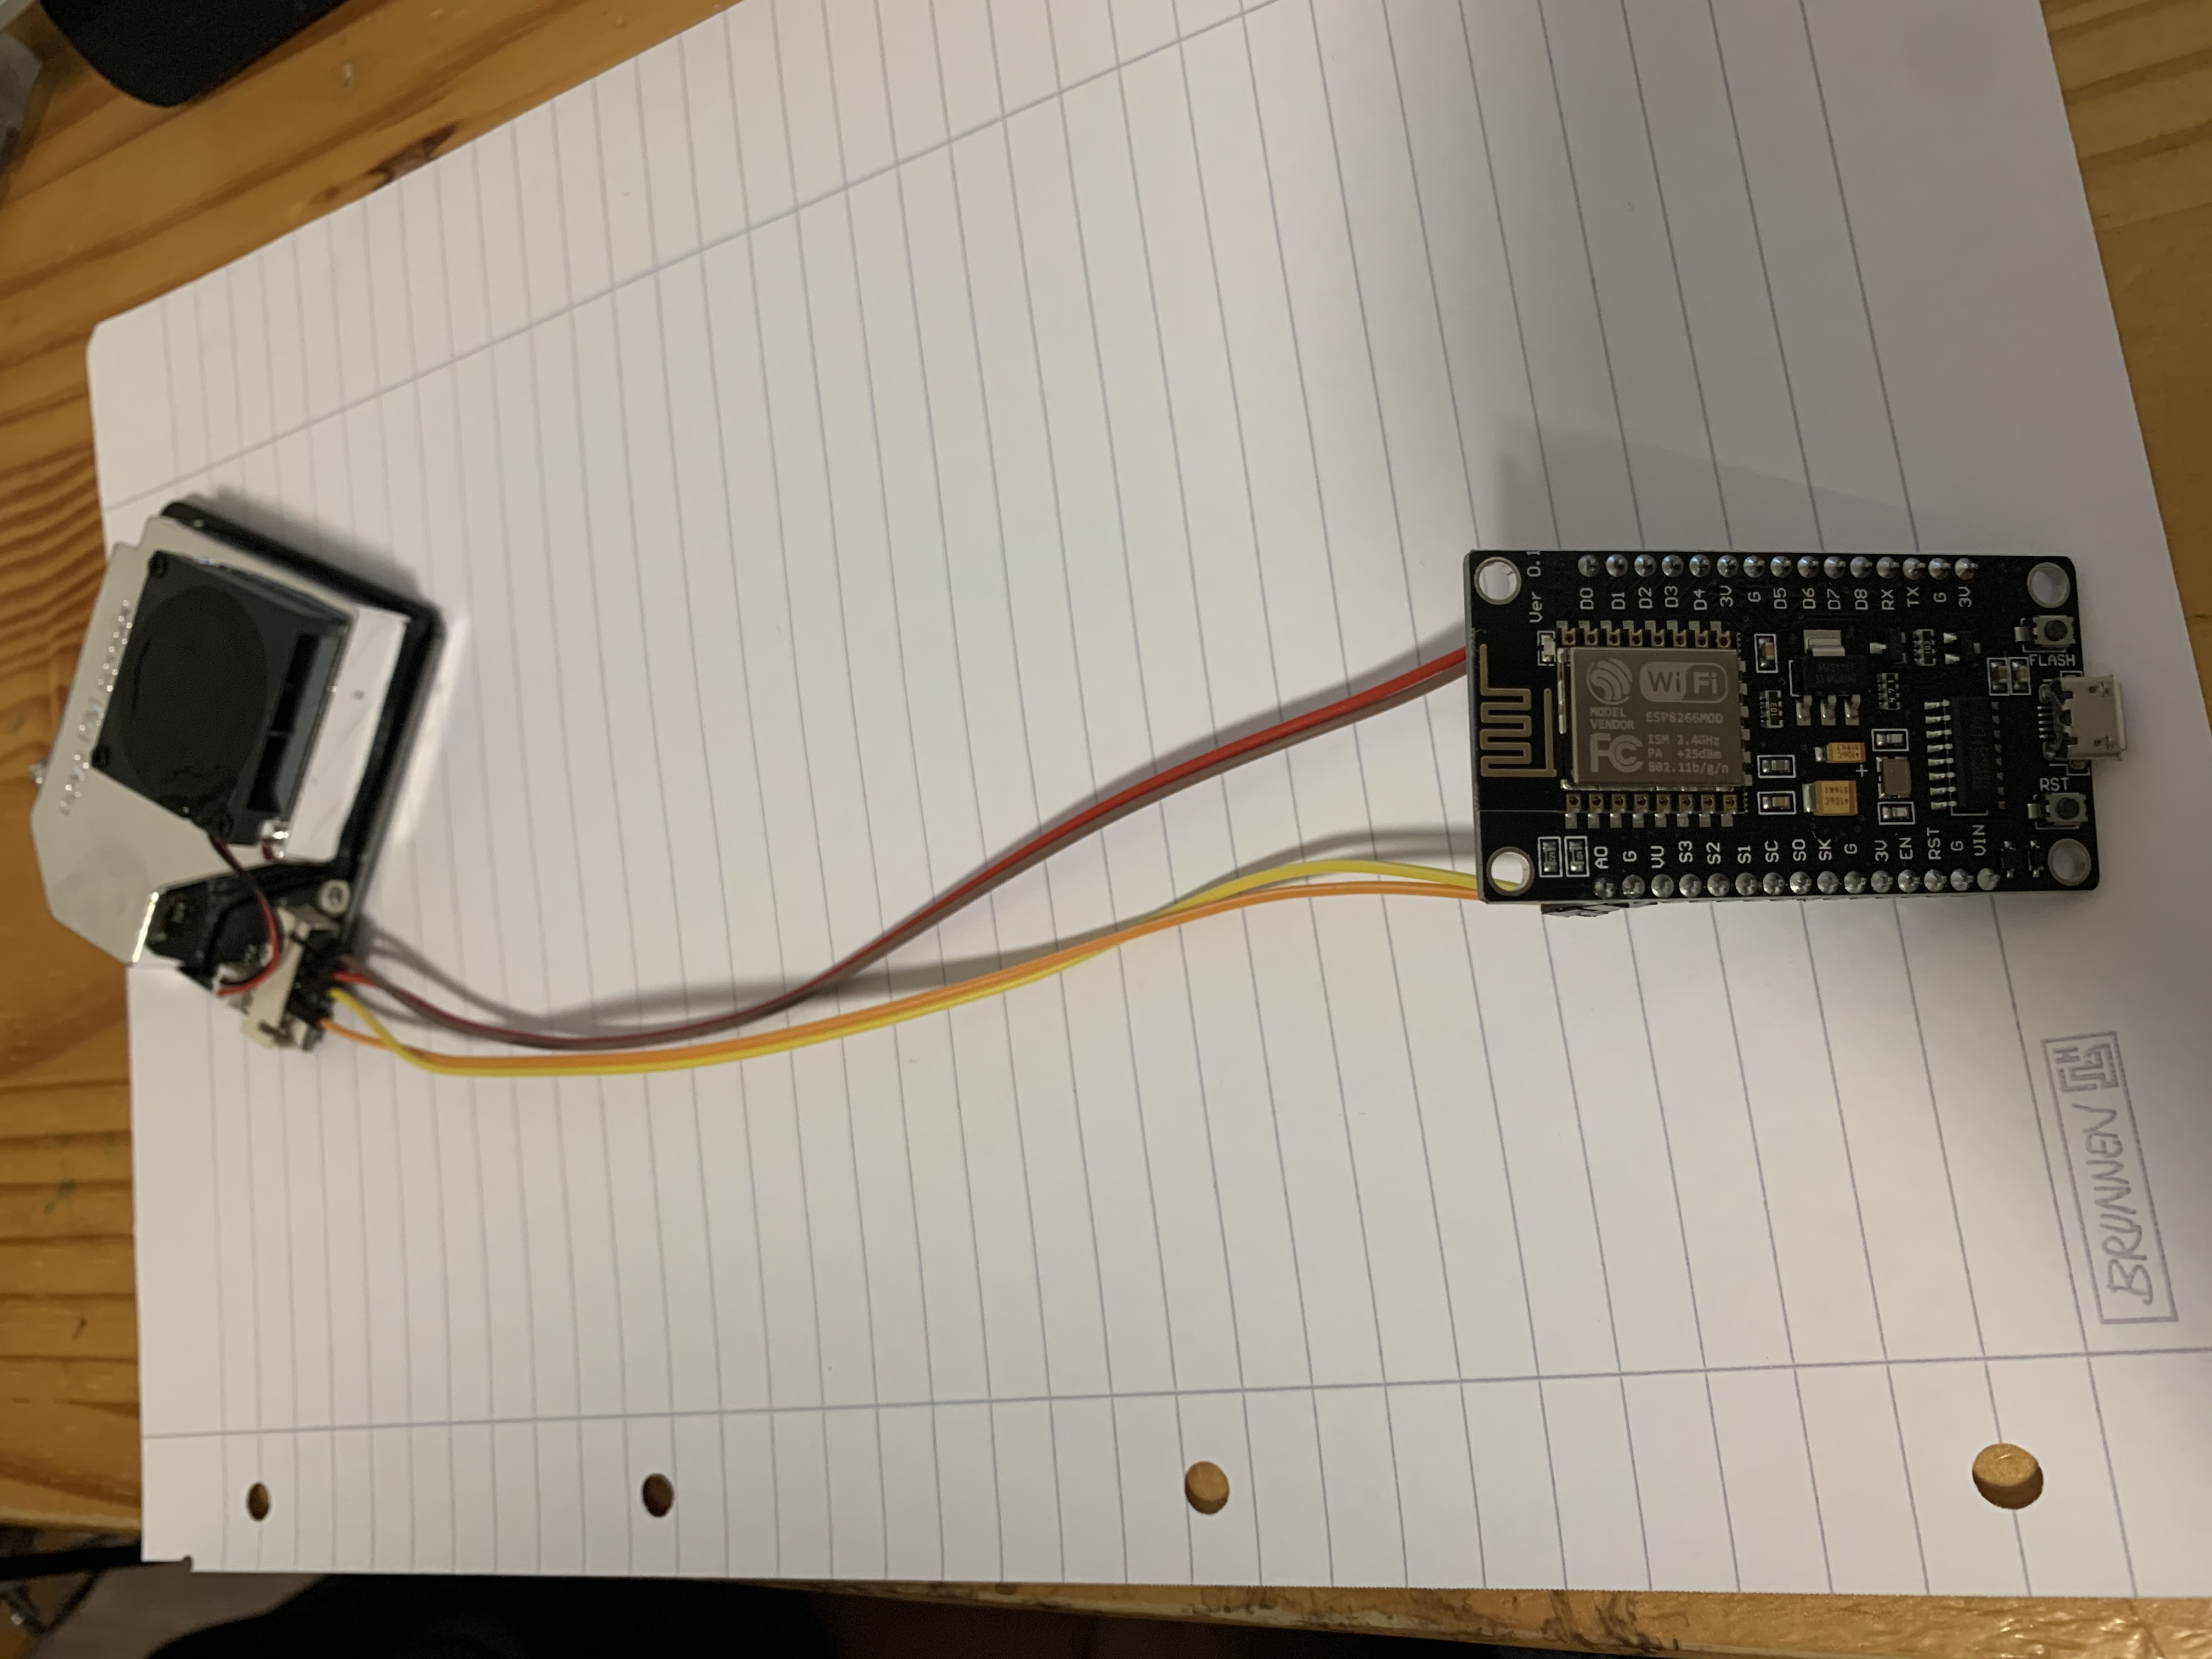
\includegraphics[width=\linewidth, angle=90]{test_day_1}
  \end{subfigure}
  \begin{subfigure}[b]{0.38\linewidth}
    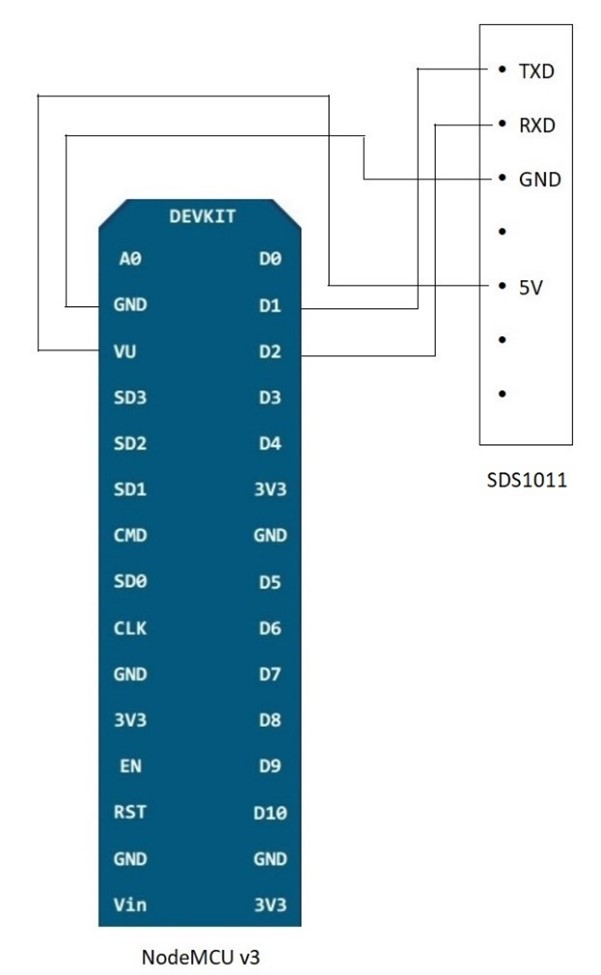
\includegraphics[width=\linewidth]{SDS011anESP}
  \end{subfigure}
  \caption{SDS011 an ESP und Verkabelung}
  \label{fig:test_day_1}
\end{figure}

Ziel: die einzelnen Komponenten zusammenbauen und testen, ob die richtig funktionieren.

Anschluss SDS011 an den ESP8266 (NodeMCU v3)

Pin sind von rechts nach links nummeriert. 

\begin{itemize}
\item SDS011 Pin 1 -> Pin D1 
\item SDS011 Pin 2 -> Pin D2 
\item SDS011 Pin 3 -> GND
\item SDS011 Pin 4 -> unbenutzt
\item SDS011 Pin 5 -> VU (NodeMCU v3) 
\item SDS011 Pin 6 -> unbenutzt
\item SDS011 Pin 7 -> unbenutzt
\end{itemize}

Danach haben wir die Station durch einen USB-Kabel mit dem Computer angeschlossen und mit dem Wifi, den der Sensor erstellt hat, verbunden. Dann haben wir den Browser geöffnet und den Link http://192.168.4.1/ eingeben. Nach dem Verbinden haben wir unter 'Konfigurieren' die SSID (Name meines WiFi-Heimnetzwerks) und das WiFi-Passwort eingegeben. Nachdem wir auf Speichern gedrückt haben, hat der Sensor neu gestartet und war auf diese Weise nicht mehr erreichbar.

\begin{figure}[H]
  \centering
  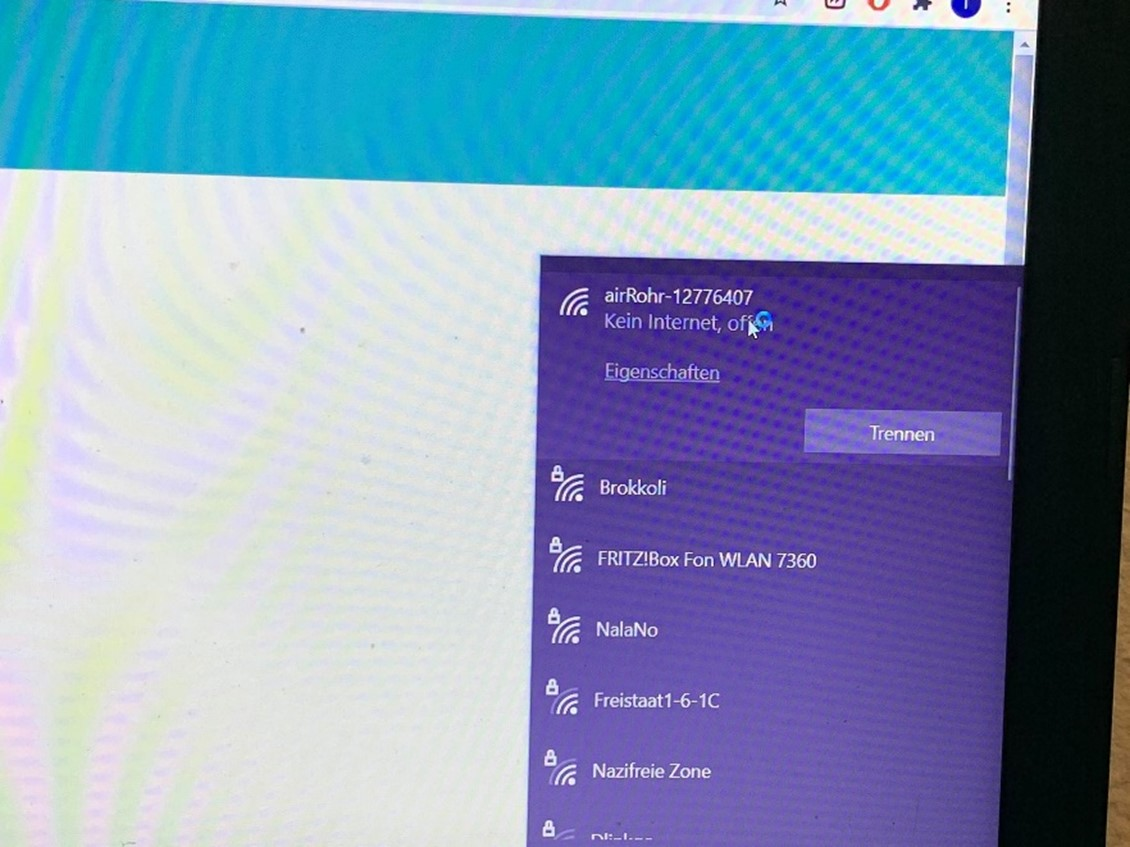
\includegraphics[width=0.8\linewidth]{WLAN}
  \caption{Name des Sensor-WLAN-Verbindung}
\end{figure}

\begin{figure}[H]
  \centering
  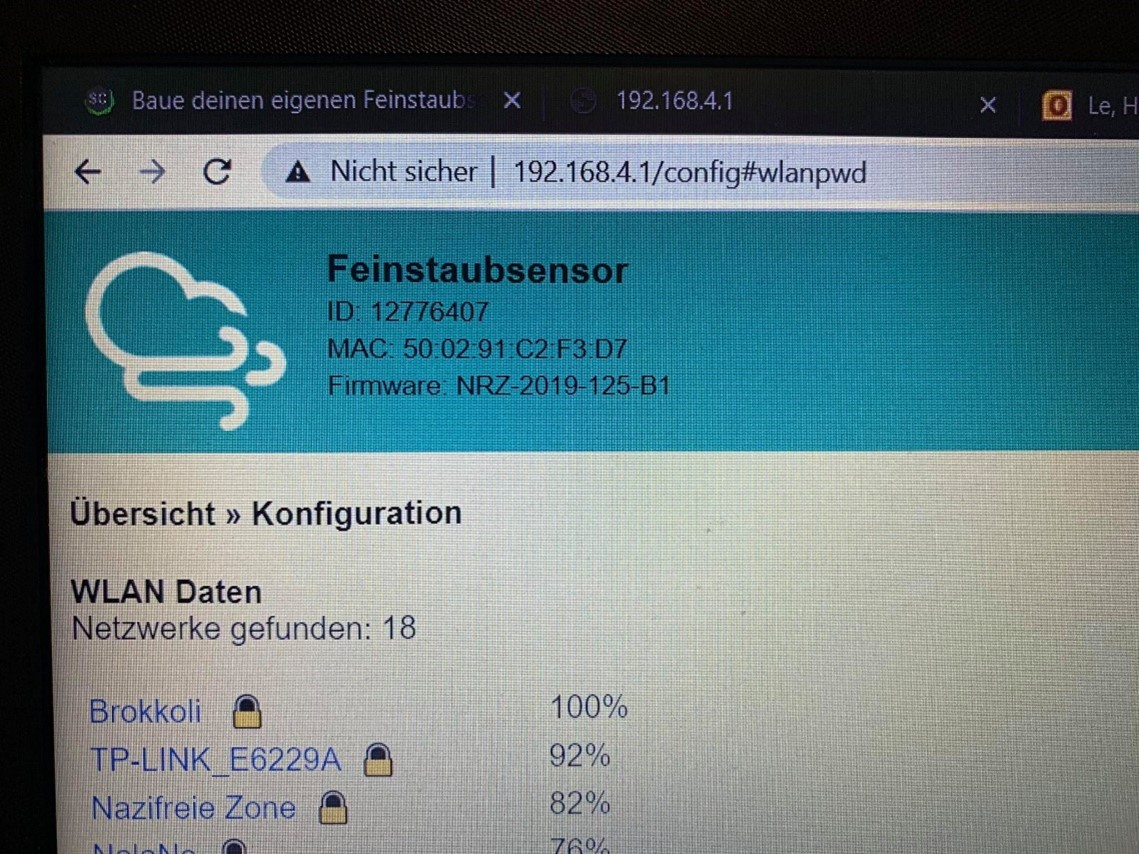
\includegraphics[width=0.8\linewidth]{konfigurationsseite}
  \caption{WLAN Konfigurationsseite }
\end{figure}

Nach 10 Minuten haben wir den Wifi-Signal unter den Link \url{https://api-rrd.madavi.de/grafana/d/Fk6mw1WGz/wifi-signal?orgId=1&var-chipID=} getestet und die Sensordaten mit ID: 12776407 unter den Link \url{https://api-rrd.madavi.de/grafana/d/GUaL5aZMz/pm-sensors?orgId=1&theme=light&var-chipID=} probiert. 

\begin{figure}[H]
  \centering
  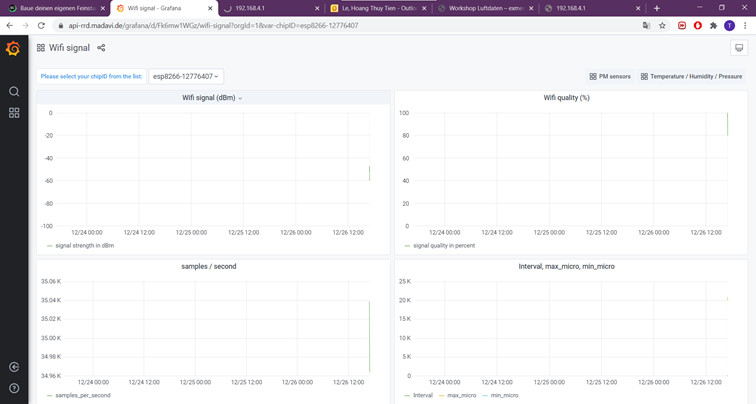
\includegraphics[width=0.8\linewidth]{versuch1_wlan}
  \caption{Wifi Signal}
\end{figure}

\begin{figure}[H]
  \centering
  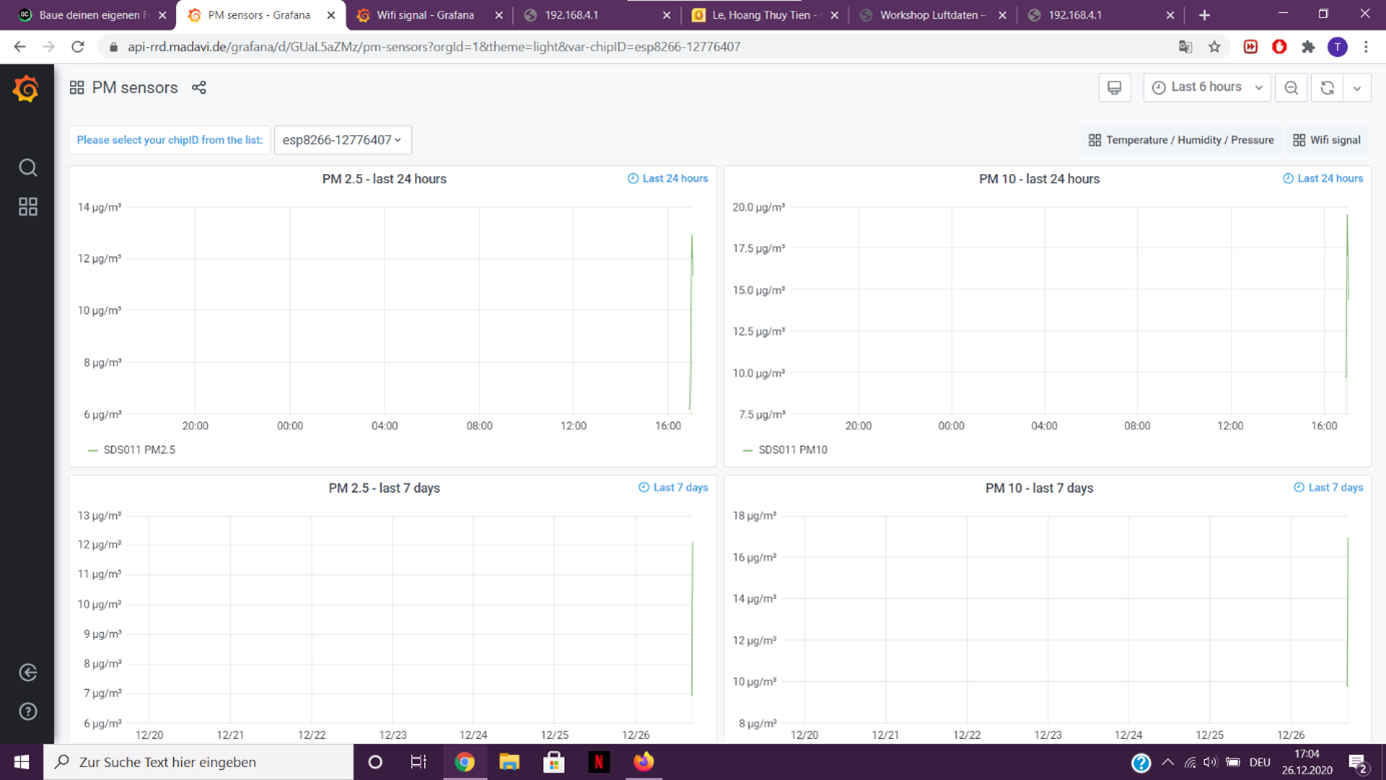
\includegraphics[width=0.8\linewidth]{versuch1_pm}
  \caption{Feinstaubsmessungen wurden im Frau Les Zimmer gemessen}
\end{figure}

\subsection{Versuche 2: Alle Bausätze bauen, mit DHT22 Sensor anschließen}

\textbf{Anschluss des DHT22 an den ESP8266 (NodeMCU v3)}

Der benutzte DHT22 hat 3 Pins und wird mit dem NodeMCU verbunden. Pins sind von links nach rechts nummeriert:

\begin{itemize}
  \item DHT22 Pin 1 -> Pin 3V3 (3.3V) 
  \item DHT22 Pin 2 -> Pin D7 (GPIO13)
  \item DHT22 Pin 3 -> Pin GND
\end{itemize}

\vspace{2cm}

\begin{figure}[h!]
  \centering
  \begin{subfigure}[b]{0.48\linewidth}
    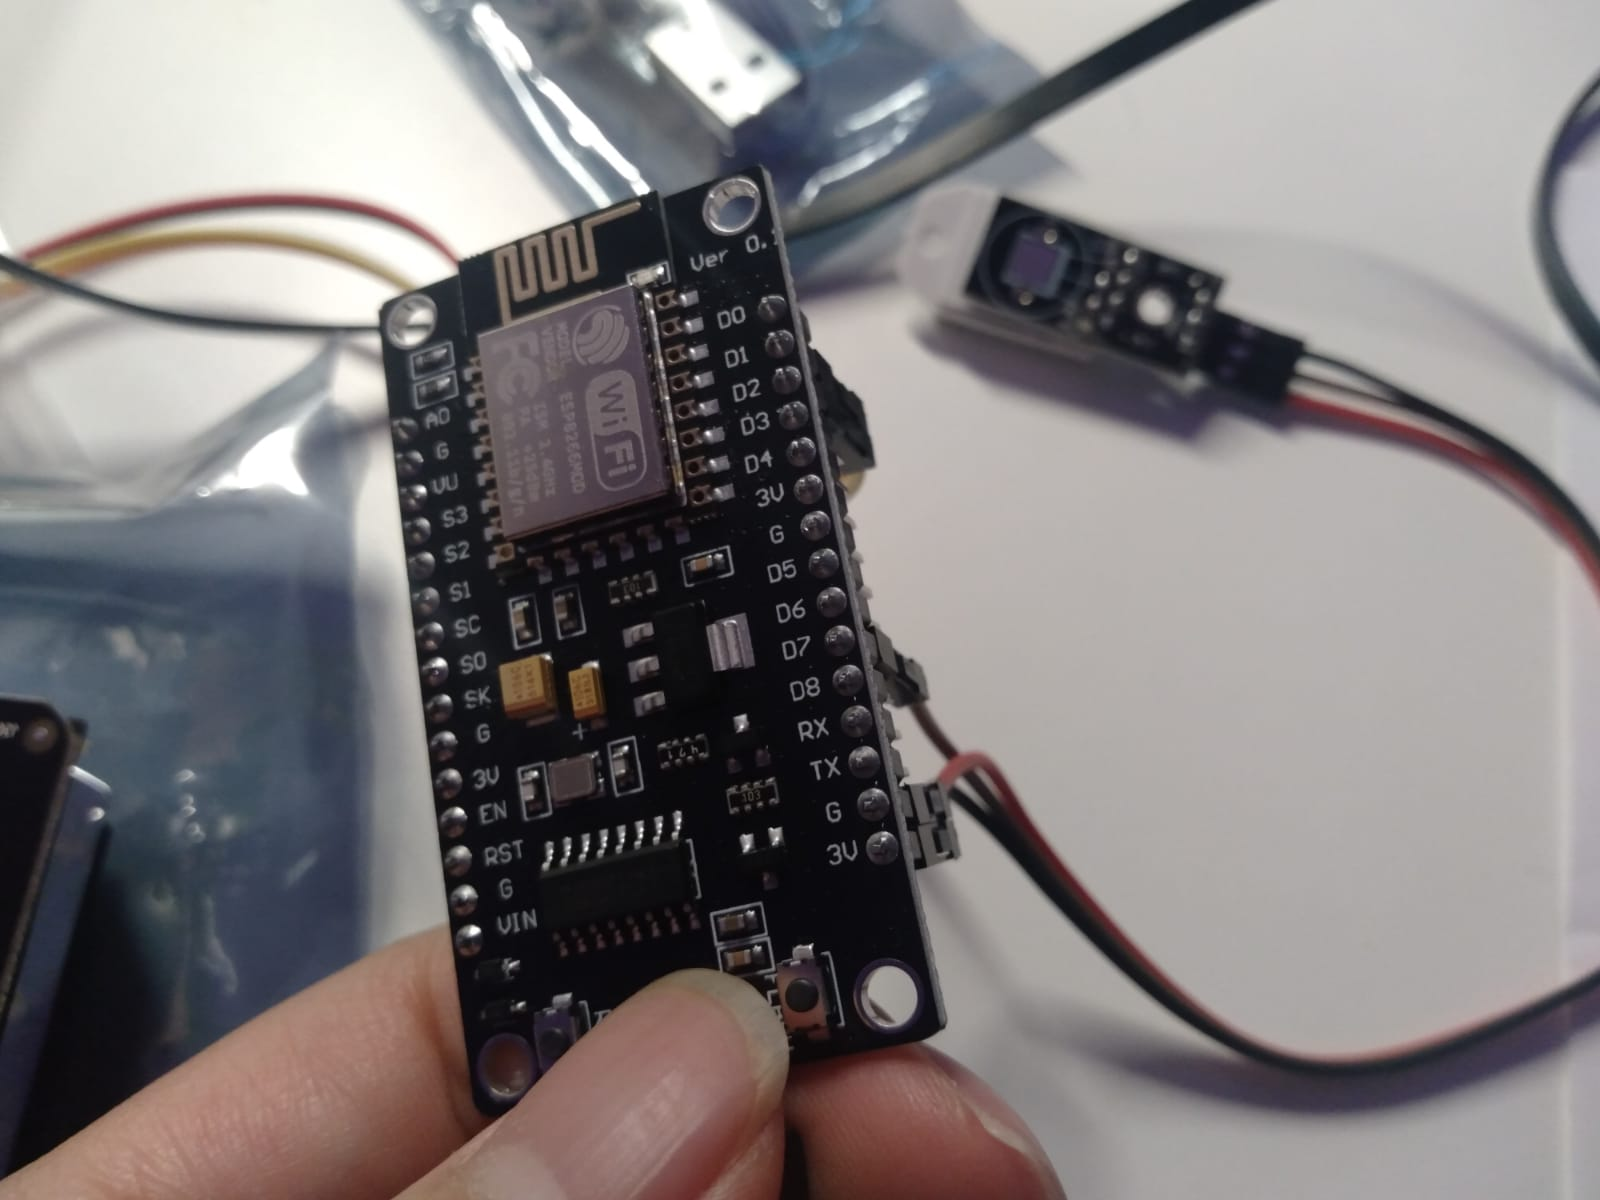
\includegraphics[width=\linewidth]{verkabelung_dht22_1}
  \end{subfigure}
  \begin{subfigure}[b]{0.48\linewidth}
    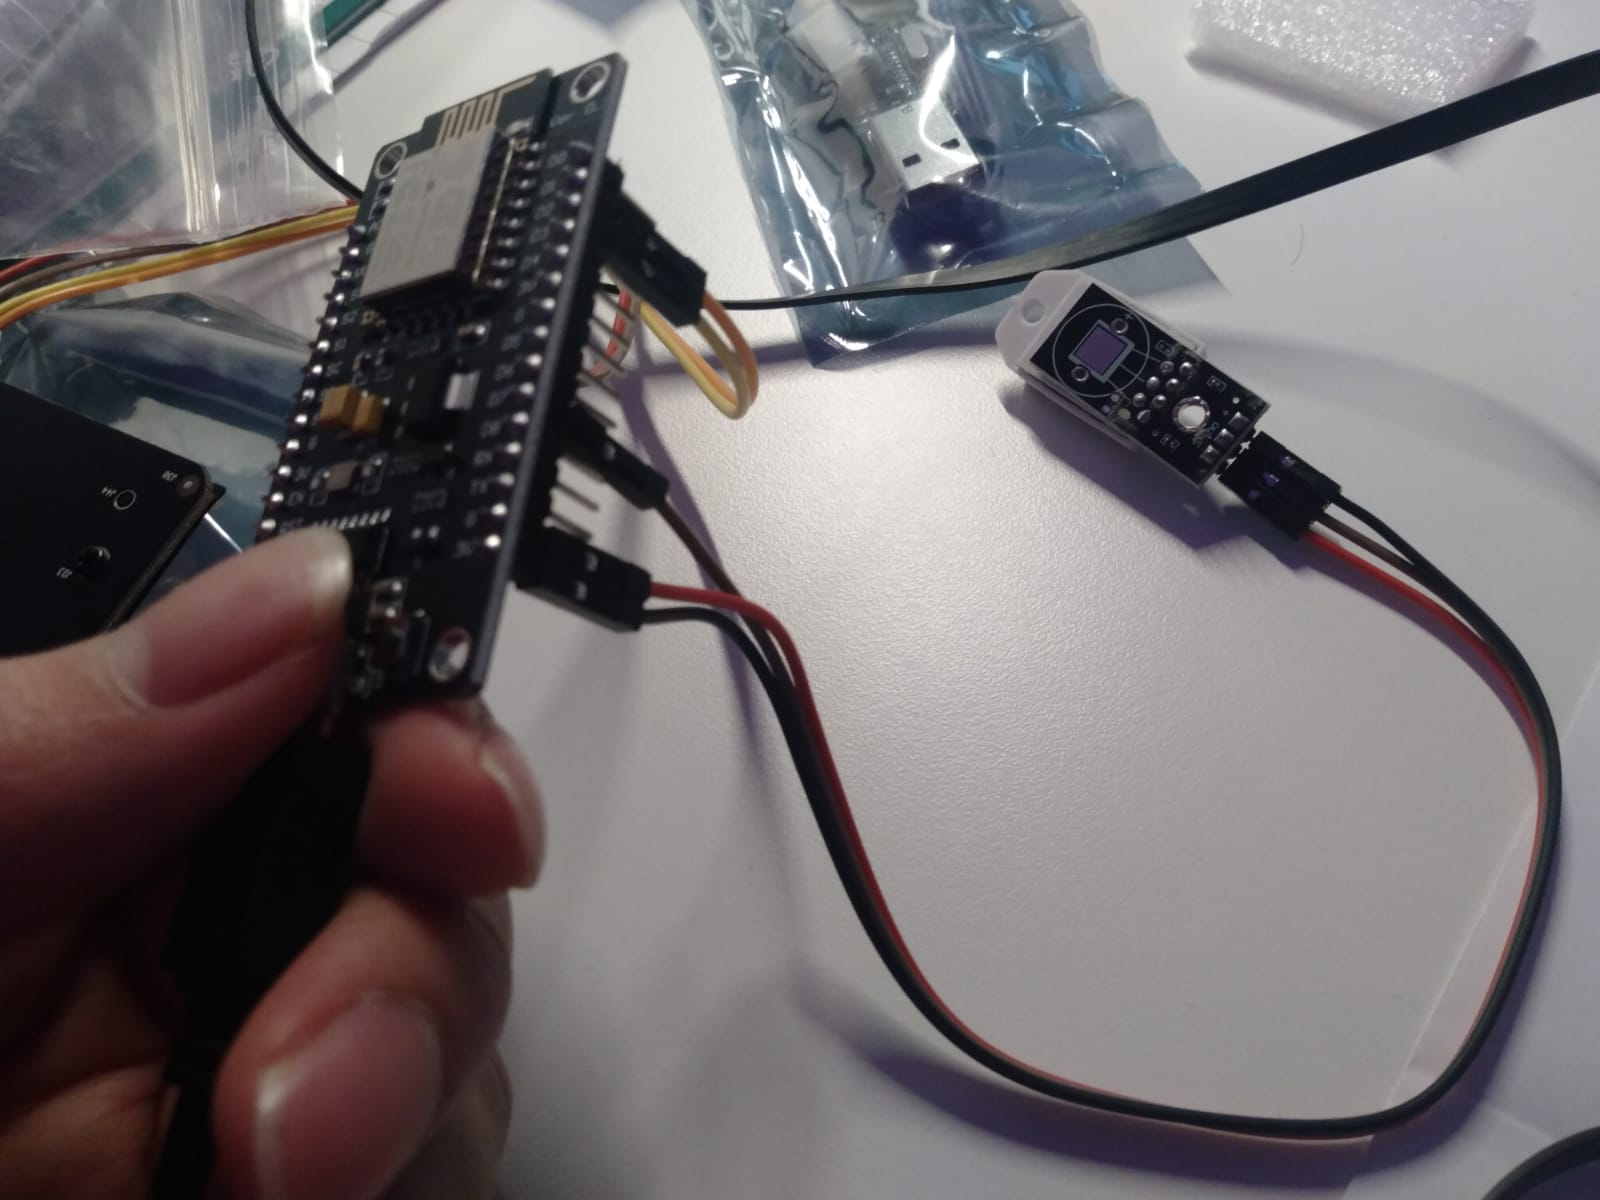
\includegraphics[width=\linewidth]{verkabelung_dht22_2}
  \end{subfigure}
  \caption{Anschluss DHT22 an NodeMCU ESP8266}
  \label{fig:dht22anNodeMCU}
\end{figure}

\begin{figure}[h!]
	\centering
	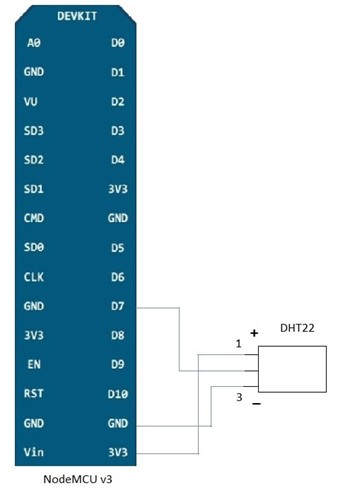
\includegraphics[width=0.6\linewidth]{DHT22anESP}
	\caption{Verkabelung DHT22 an ESP8266}
\end{figure}

\begin{figure}[h!]
  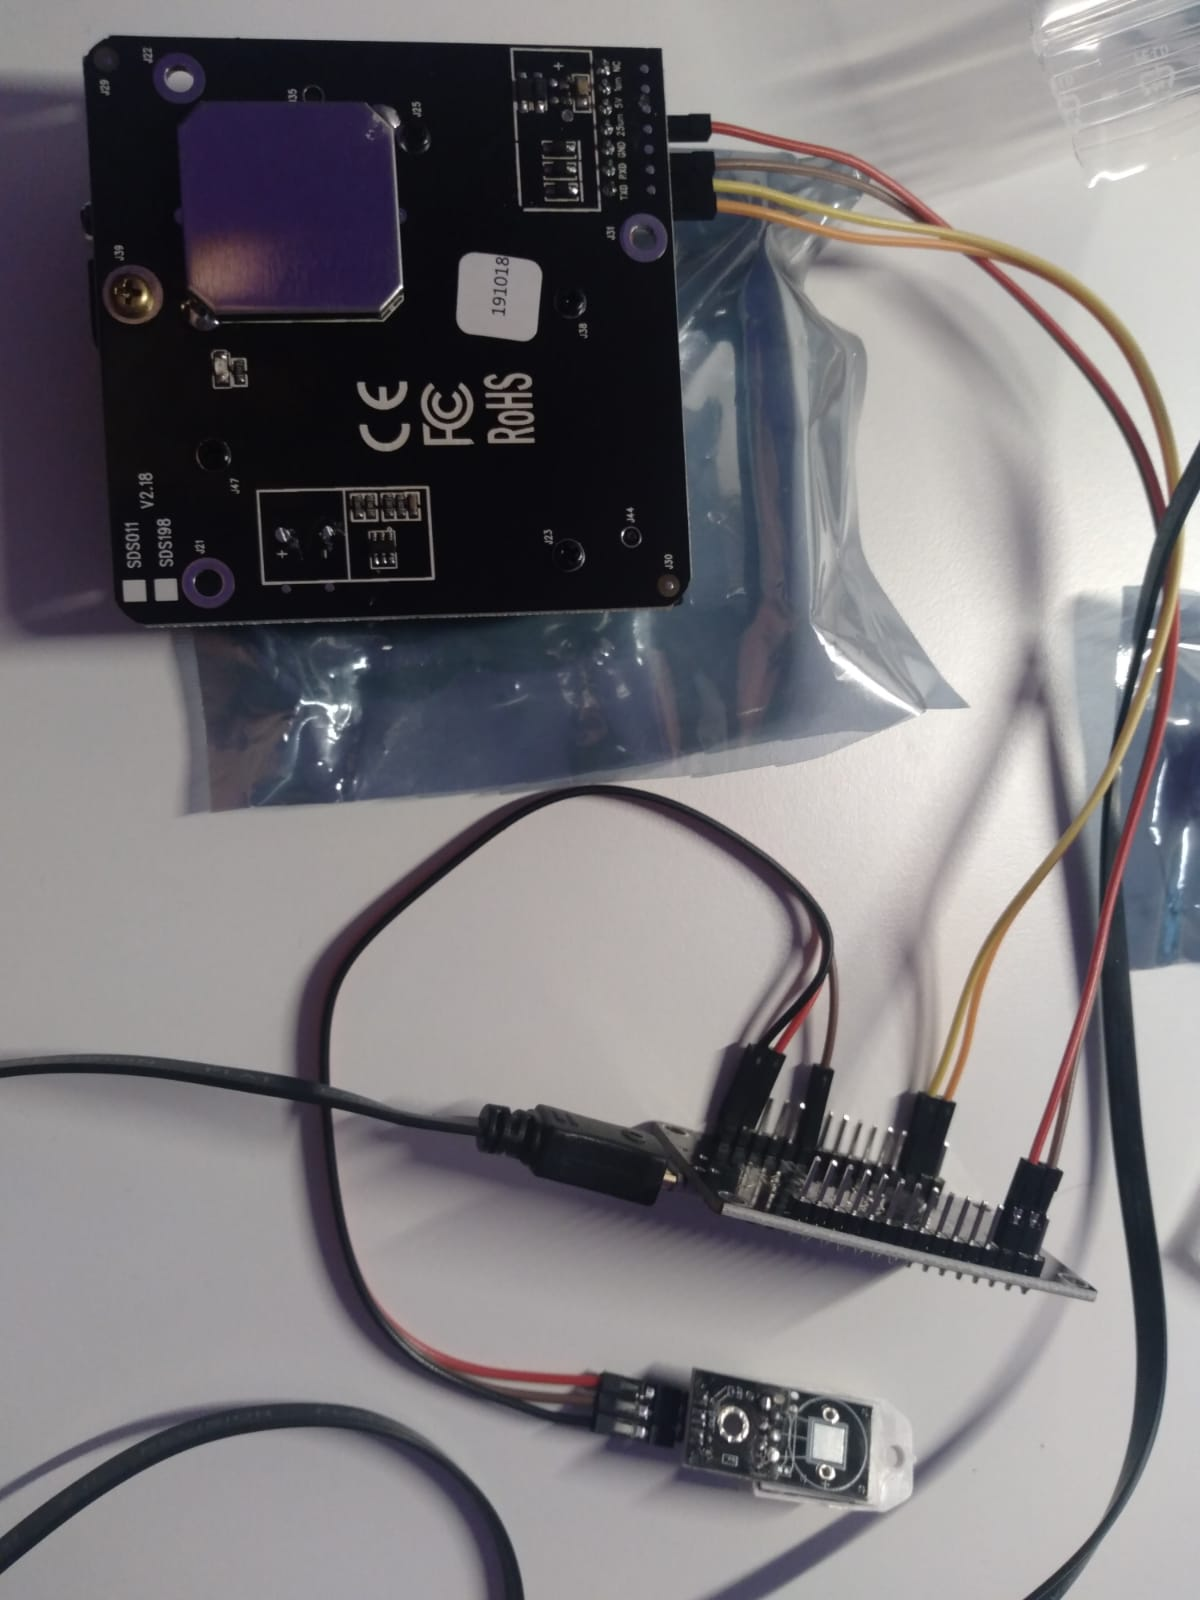
\includegraphics[width=0.6\textwidth, angle=90]{gesamt}
  \caption{Gesamtbau von NodeMCU, SDS011 und DHT22, Stromversorgung von USB-Anschluss am Rechner}
\end{figure}

\begin{figure}[H]
  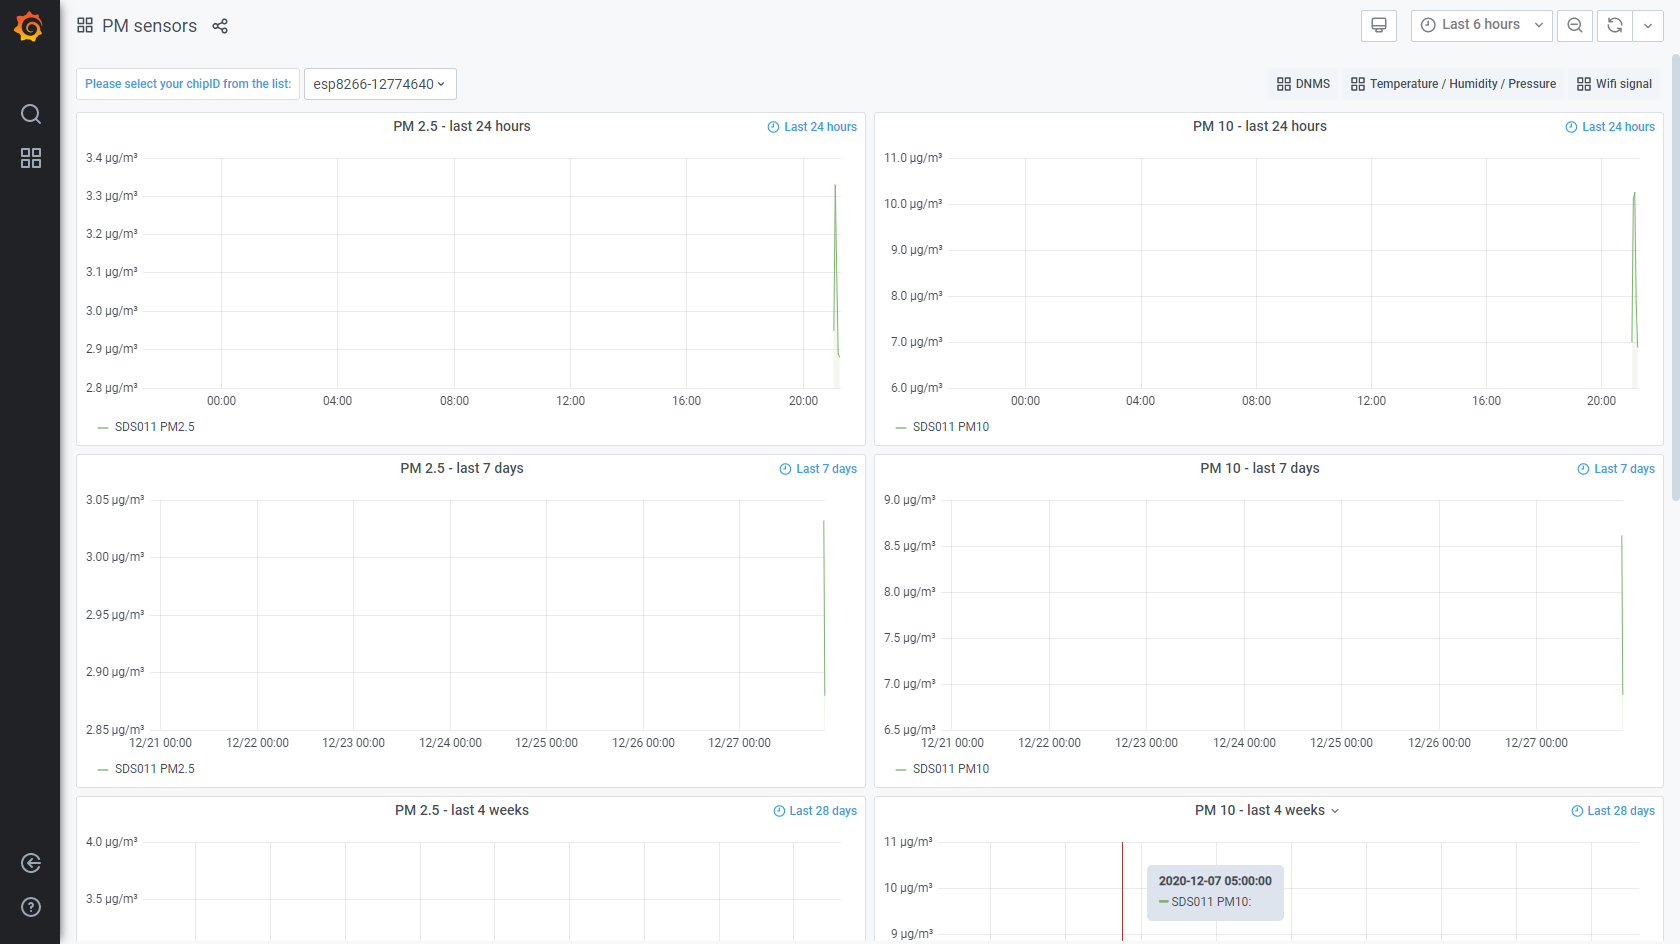
\includegraphics[width=\textwidth]{airrohr-12774640}
  \caption{airrohr-12774640}
\end{figure}

\begin{figure}[H]
  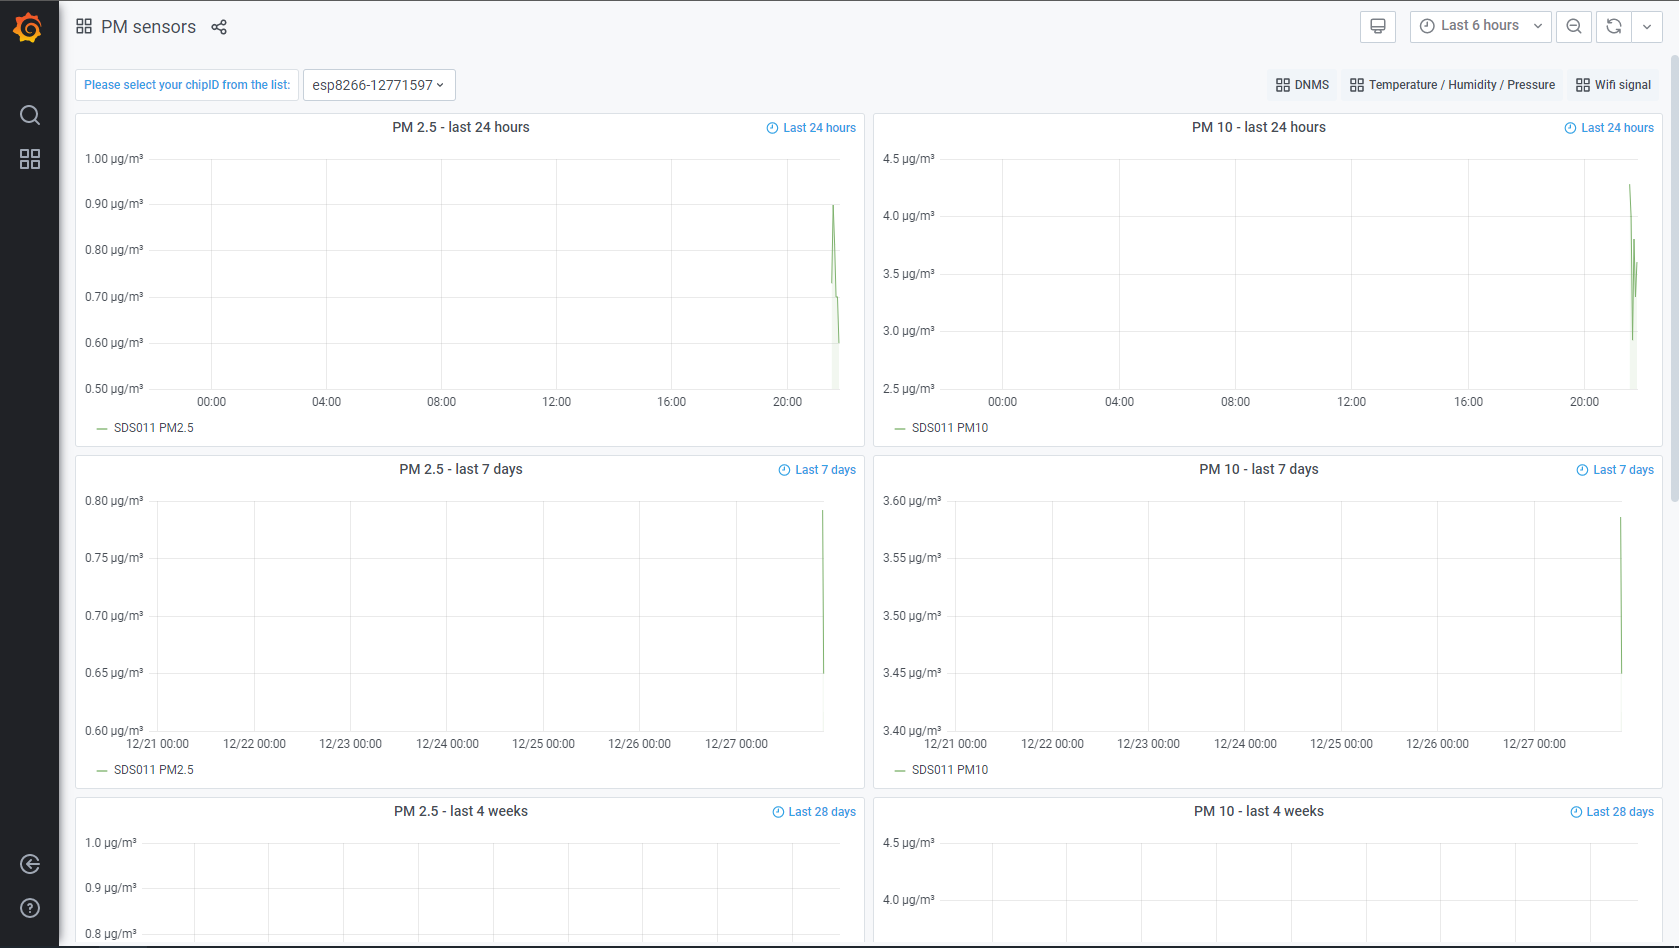
\includegraphics[width=\textwidth]{airrohr-12771597}
  \caption{airrohr-12771597}
\end{figure}

\begin{figure}[H]
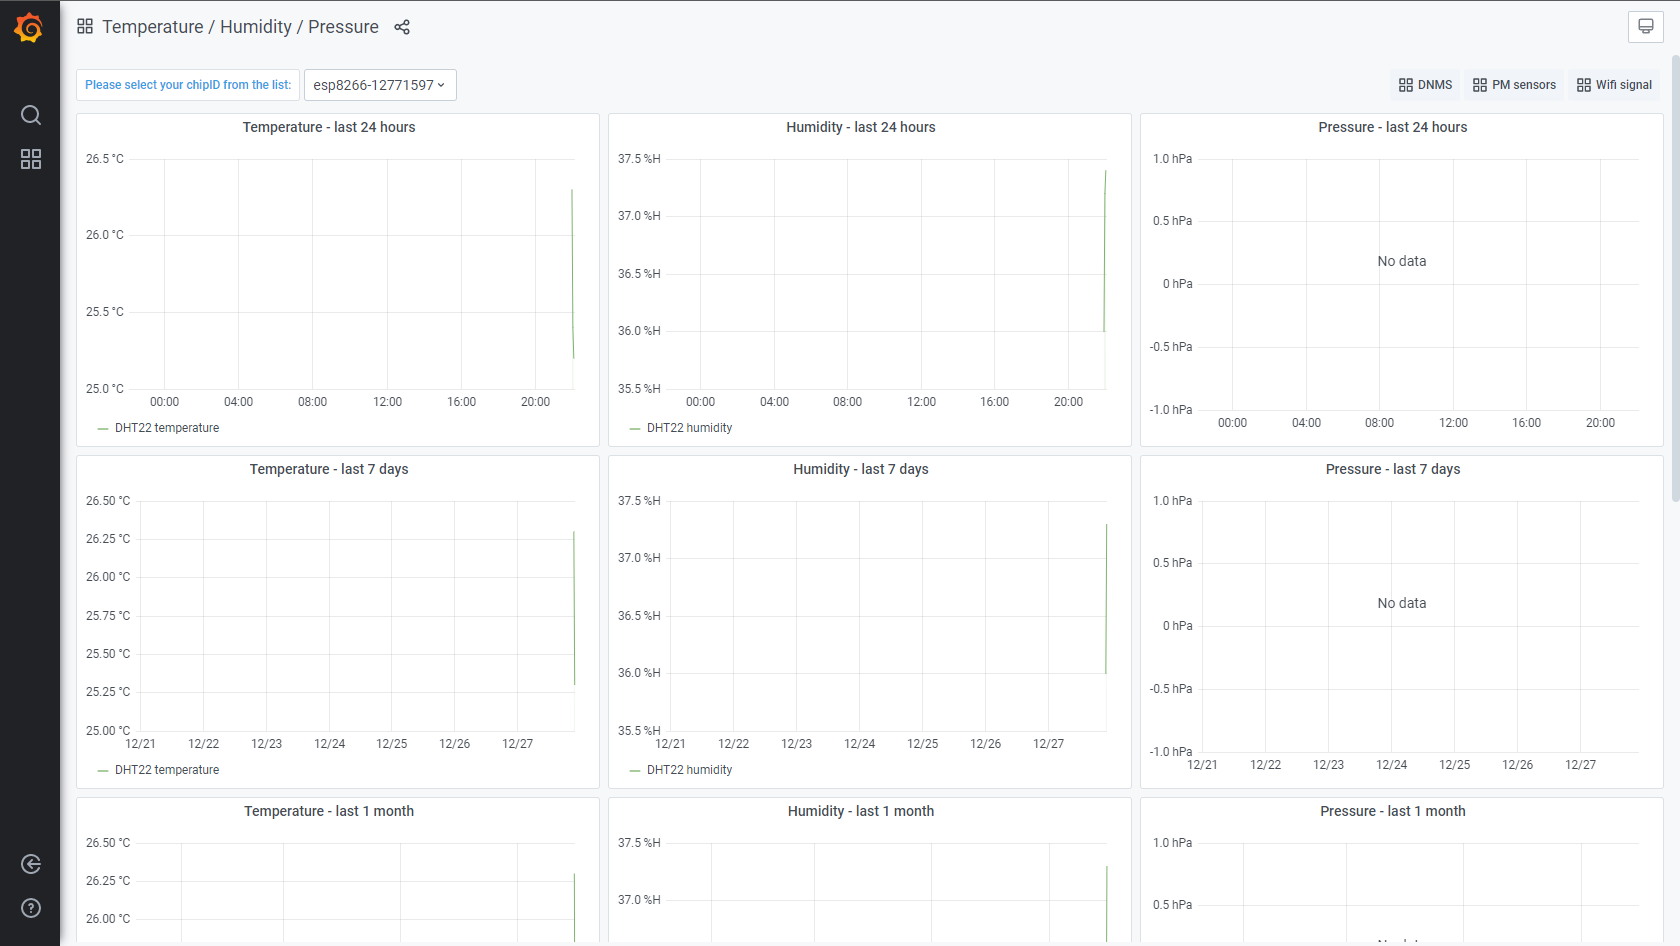
\includegraphics[width=\textwidth]{airrohr-12771597DHT22Messung}
\caption{airrohr-12771597 mit DHT22 Luftfeuchtigkeit und Temperaturmessung}
\end{figure}

\subsection{Ergebnisse}
Die Sensoren funktionieren einwandfrei und sind im gutem Zustand, nur ein NodeMCU wurde physikalisch an einem Bein ein bisschen gebogen. PIN mit Anschlüsse an Kabel sind im Grunde auch schon ganz gut verbunden.

Auf Untersuchung des Projekts von OK Lab Stuttgart(Code for Germany) wurde gesehen, dass der Endbau kein Löten von Kabeln gebraucht wurde. Aber es ist machbar von unterer Seite des NodeMCU.

\section{Einkaufliste}
\subsection{Gesamte Aufbau}
Nach Einleitung aus \cite{airrohrbau} und mehr Infos auf \cite{wiki} haben wir eine Liste:

\begin{itemize}
  \item NodeMCU ESP8266 CPU/WLAN
  \item SDS011 Feinstaub-Sensor
  \item DHT22 3-PIN, Temperatur und Feuchtigkeit
  \item Kabeln
  \item USB-Kabel z.B.: flach 2m Micro-USB
  \item Stromversorgung USB (Stecker)
  \item Kabelbinder
  \item Flexibler Schlauch, wenn möglich nicht transparent, Durchmesser 6 mm, Länge ca. 20cm Baumarkt
  \item Witterungsschutz, Marley Silent HT Bogen DN 75 87° \url{https://www.bauhaus.info/ht-rohre/marley-ht-bogen/p/13625028}
\end{itemize}

Einleitung Zusammenbau der Komponenten (Montage Einzelteile): 

\url{https://github.com/opendata-stuttgart/meta/wiki/Zusammenbau-der-Komponenten-(Montage-Einzelteile)}

\begin{figure}[H]
  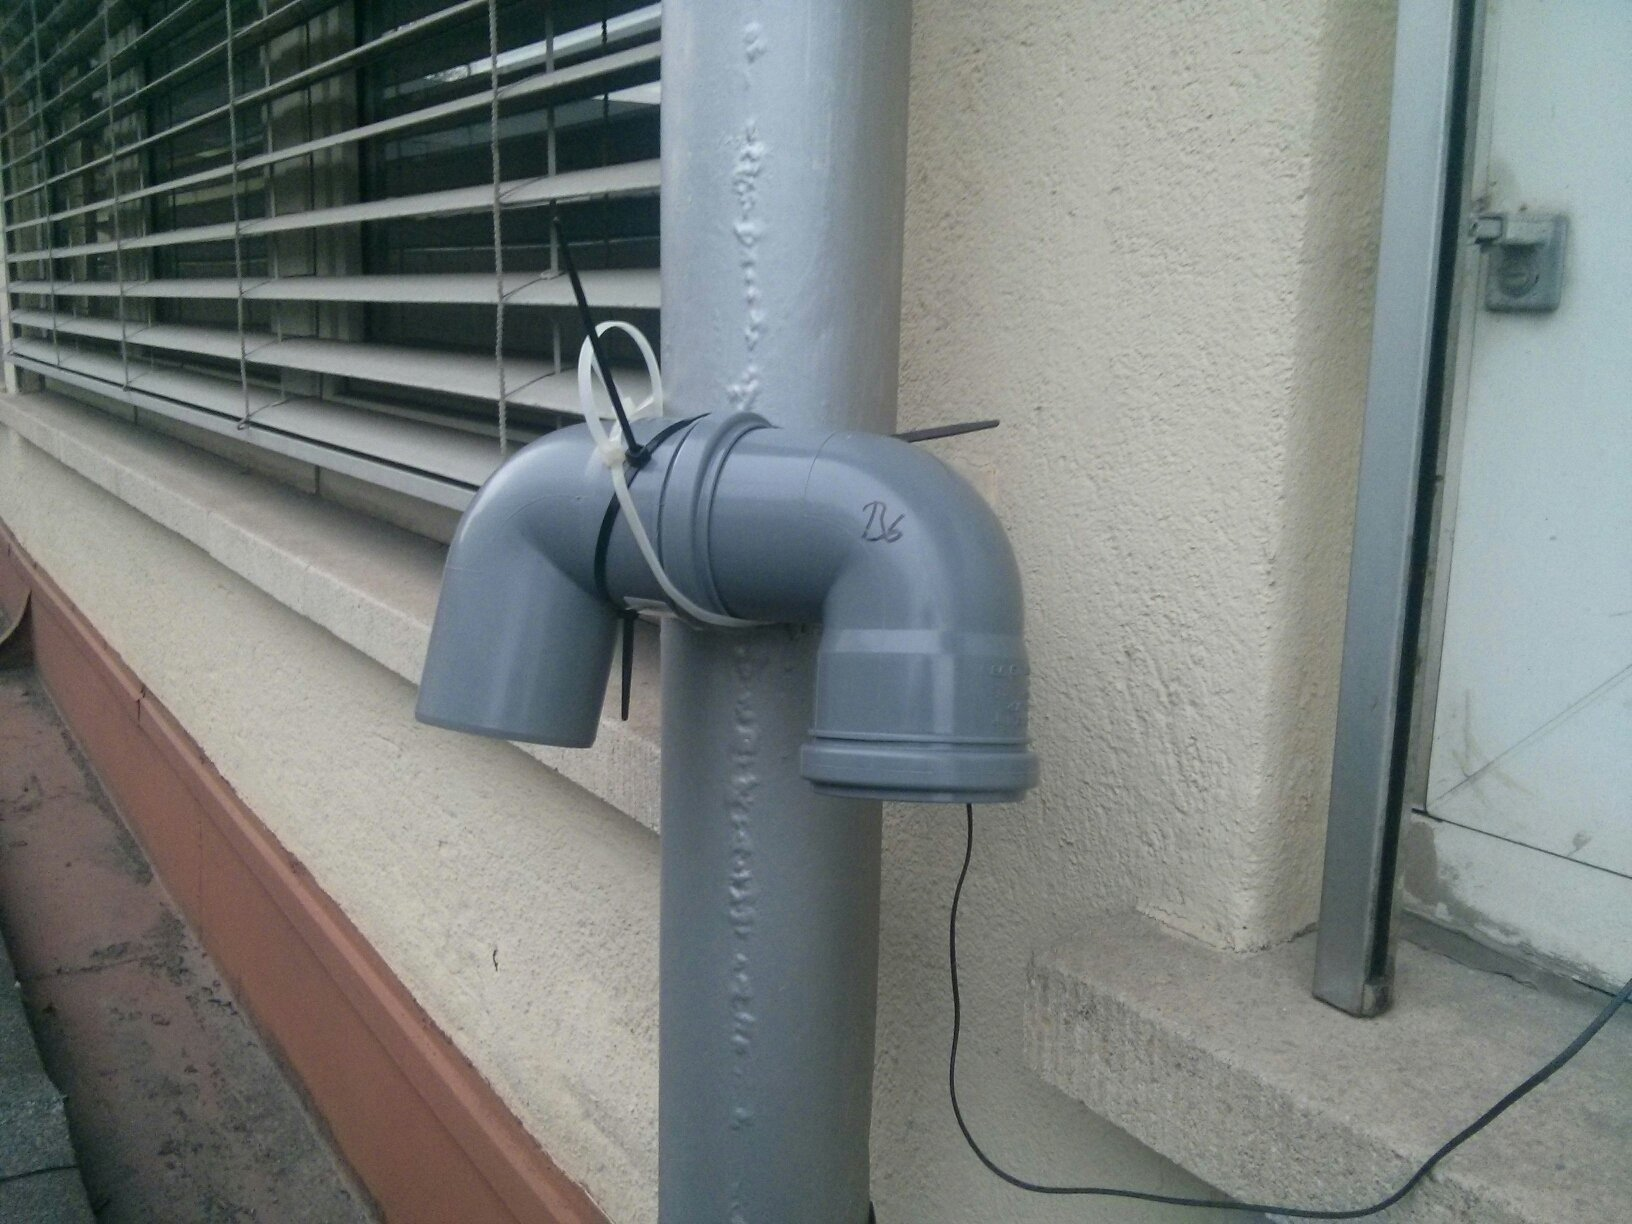
\includegraphics[width=0.8\linewidth]{endbau}
  \caption{Beispiel Endbau einer Messstation}
\end{figure}

\subsection{Noch zu kaufen bzw. suchen}
\textbf{Vorgeschlagen von \cite{bezugsquellen}}

\textit{Vorgeschlagener Ort des Kaufens: Baumarkt}

\begin{itemize}
  \item Stromversorgung USB (Stecker) (Menge: 3 mal oder 1 mal + USBHub) *für Einsetzen im Feld (z.B auf dem Dach)
  \item Wetterschutz: Gehäuse aus zwei Marley Silent HT Rohr-Bogen (DN 75 87°). etwa je 2 Euro. \url{https://www.bauhaus.info/ht-rohre/marley-ht-bogen/p/13625028} Menge: 6 Stück
  \item Schutz vor Tierchen: Luftdurchlässiges Netz/Gitter, das die Rohrbogen abschließt. Menge: 6 Stück
  \item Plastikschlauch, z.B. aus PVC, ca. 20cm, Innen-Durchmesser mindestens 6mm, möglichst nicht transparent. Menge: 3 Stück
  \item Kabelbinder zur Befestigung der Platinen miteinander und zum Fixieren der Kabel. (optional)
  \item Panzerband (Ducktape/Gaffertape) oder Heißklebepistole. (optional)
\end{itemize}

\section{Zukünftige Planen}

Nachdem wir die Bauteile gekauft haben, fängt der Aufbau der Module mit Messrohr(Plastikschlauch, Umhüllung(Wetterschutzrohr)) an.
Danach weitere Testausbauen können durchgeführt werden. Ideen sind erstmal von \cite{wiki} genommen und verarbeiten. Möglicherweise eine selbsterstellte Messdatensmonitoring von CSV-Dateien, die jeden Tag um 8 Uhr morgen von NodeMCU nach Sensor.Community API-Server gesendet werden.

\newpage
%% printbibliography
\printbibliography[title={Literatursverzeichnis}]
\addcontentsline{toc}{section}{Literatursverzeichnis}
%% Umcomment these 4 lines to input \bibliography manually from other file
%% \newpage
%% \newpage
%% \input{bibliography}

%% \printglossary[type=\acronymtype,title={List of Abbreviations}]
%% \addcontentsline{toc}{section}{List of abbreviations}
%% \newpage
%% \thispagestyle{plain}
\textbf{Declaration of originality}

\vspace{6pt}

I hereby declare that this term paper and the work reported herein was composed by and originated entirely from me. Information derived from published and unpublished work of others has been acknowledged in the text and references are given in the list of references. 

\begin{flushright}
	\today

	Duy Nguyen
\end{flushright}

%% \addcontentsline{toc}{section}{Declaration of originality}
\end{document}
